% Requires \usepackage{graphicx}. Copy the PDF beside the manuscript or
% adjust its path. Use figure* for a full-width figure in a two-column paper.
\begin{figure*}[t]
  \centering
  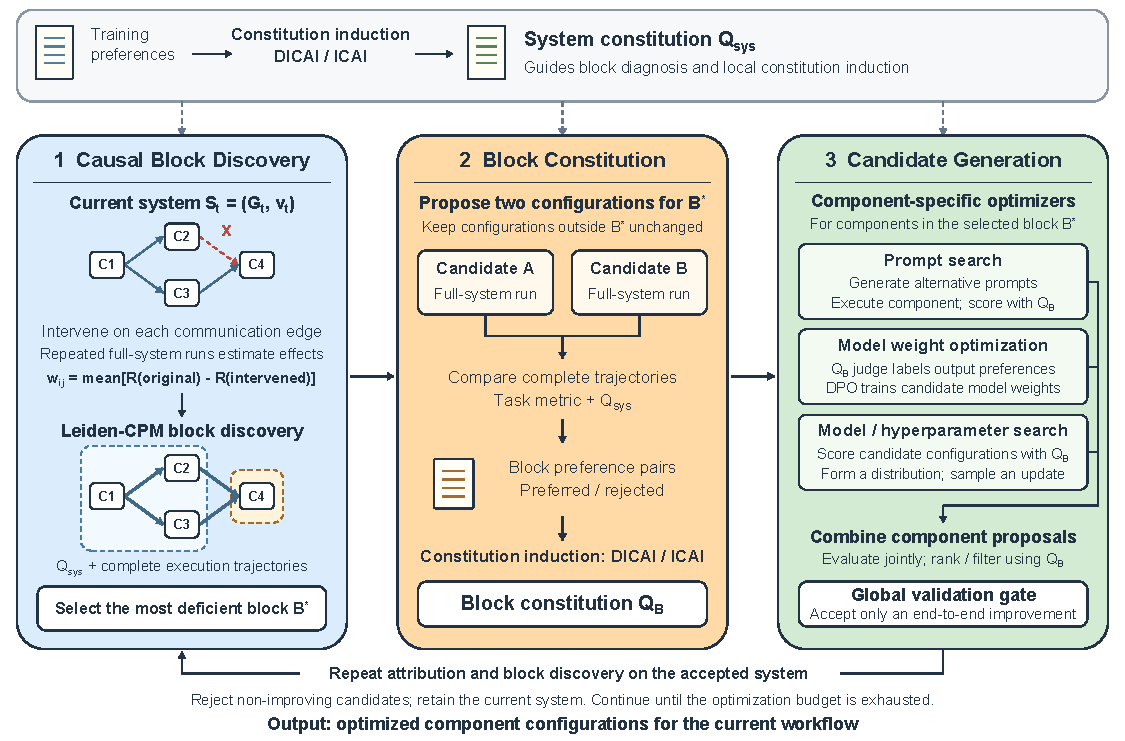
\includegraphics[width=\textwidth]{output/pdf/caiso_overview.pdf}
  \caption{Overview of the proposed compound AI system optimization method.
  A system constitution induced from training preferences guides three stages.
  (1) Repeated edge interventions estimate causal effects, Leiden-CPM partitions
  the current workflow, and constitution-guided trajectory diagnosis selects
  a deficient block.
  (2) Full-system comparisons of block configurations provide preferences for
  a local constitution. Component-specific optimizers generate alternative
  prompts, preference-trained weights, or sampled model and parameter
  configurations. These proposals are combined within the selected block,
  ranked or filtered using its constitution, and accepted only when they
  improve end-to-end performance.
  (3) After $K$ accepted block updates or a performance plateau, a workflow
  generator uses the current DAG, fixed component library, and system
  constitution to propose one structural modification, followed by brief
  adaptation of affected blocks. Optimization repeats until the budget
  is exhausted; an accepted structural change also refreshes the system
  constitution. Graphs and partitions are illustrative.}
  \label{fig:caiso-overview}
\end{figure*}
